\section{Running \Queso\ in parallel}
\begin{frame}[fragile]{Parallel \Queso}
  \begin{itemize}
    \item Have been running with \texttt{./binary inputfile.txt}
    \item This is equivalent to \texttt{mpirun -np 1 ./binary inputfile.txt}
    \item Want to do \texttt{mpirun -np N ./binary inputfile.txt}
    \item \texttt{N = 2} will tell \Queso\ to give the sampler two processes
    \item But still only one chain produced!  Why?
    \item The usecase for this would be if the \emph{forward problem} needed
      two processes per evaluation
  \end{itemize}
\end{frame}

\begin{frame}{Parallel \Queso}
  \begin{figure}
    \centering
    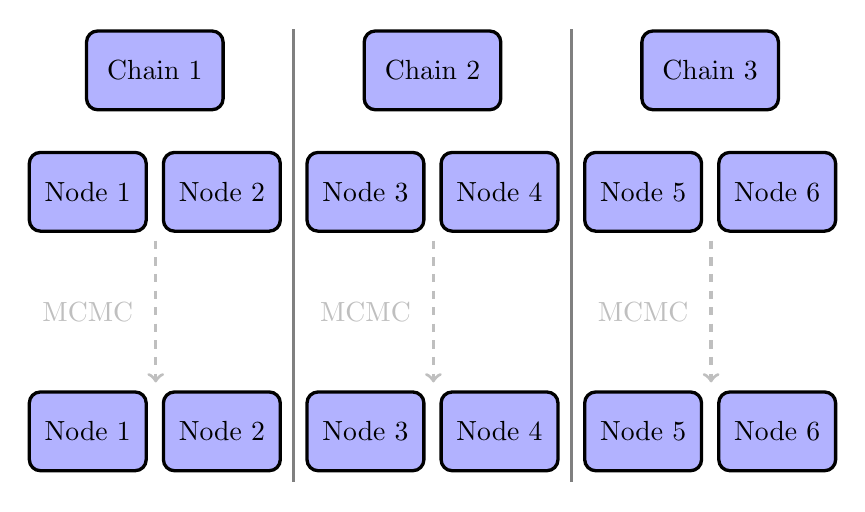
\begin{tikzpicture}[
      desc/.style={
        rectangle,
        rounded corners,
        draw=black,
        very thick,
        text centered,
        text width=8cm,
        minimum height=10mm,
        fill=blue!30
      }
    ]

    % Chains
    \node[desc, text width=1.5cm, anchor=east, xshift=1.75cm] (Chain1) {Chain 1};
    \node[desc, text width=1.5cm, anchor=west, xshift=1.75cm] (Chain2) at (Chain1.east) {Chain 2};
    \node[desc, text width=1.5cm, anchor=west, xshift=1.75cm] (Chain3) at (Chain2.east) {Chain 3};

    % Separators
    % \draw [very thick,-,gray] (Chain1.south west) ++(0,-0.4) -- ++(0,-5);
    \draw[very thick,-,gray] (Chain1.north east) ++(0.875,0) -- ++(0,-5.75);
    \draw[very thick,-,gray] (Chain2.north east) ++(0.875,0) -- ++(0,-5.75);

    % Nodes in chain 1
    \node[desc, text width=1.25cm, anchor=north east, xshift=8mm, yshift=-5mm] (Node1) at (Chain1.south west) {Node 1};
    \node[desc, text width=1.25cm, anchor=north west, xshift=-8mm, yshift=-5mm] (Node2) at (Chain1.south east) {Node 2};

    % Nodes in chain 2
    \node[desc, text width=1.25cm, anchor=north east, xshift=8mm, yshift=-5mm] (Node3) at (Chain2.south west) {Node 3};
    \node[desc, text width=1.25cm, anchor=north west, xshift=-8mm, yshift=-5mm] (Node4) at (Chain2.south east) {Node 4};

    % Nodes in chain 3
    \node[desc, text width=1.25cm, anchor=north east, xshift=8mm, yshift=-5mm] (Node5) at (Chain3.south west) {Node 5};
    \node[desc, text width=1.25cm, anchor=north west, xshift=-8mm, yshift=-5mm] (Node6) at (Chain3.south east) {Node 6};

    % Nodes in chain 1 after mcmc iter
    \node[desc, text width=1.25cm, anchor=north, yshift=-2cm] (Node11) at (Node1.south) {Node 1};
    \node[desc, text width=1.25cm, anchor=north, yshift=-2cm] (Node21) at (Node2.south) {Node 2};

    % Nodes in chain 2 after mcmc iter
    \node[desc, text width=1.25cm, anchor=north, yshift=-2cm] (Node31) at (Node3.south) {Node 3};
    \node[desc, text width=1.25cm, anchor=north, yshift=-2cm] (Node41) at (Node4.south) {Node 4};

    % Nodes in chain 3 after mcmc iter
    \node[desc, text width=1.25cm, anchor=north, yshift=-2cm] (Node51) at (Node5.south) {Node 5};
    \node[desc, text width=1.25cm, anchor=north, yshift=-2cm] (Node61) at (Node6.south) {Node 6};

    % MCMC arrows
    \draw[very thick,->,dashed,lightgray] (Node1.south east) ++(0.1,-0.1) -- ++(0,-1.8);
    \draw[very thick,->,dashed,lightgray] (Node3.south east) ++(0.1,-0.1) -- ++(0,-1.8);
    \draw[very thick,->,dashed,lightgray] (Node5.south east) ++(0.1,-0.1) -- ++(0,-1.8);

    % MCMC text
    \node[yshift=-1cm,text=lightgray] at (Node1.south) {MCMC};
    \node[yshift=-1cm,text=lightgray] at (Node3.south) {MCMC};
    \node[yshift=-1cm,text=lightgray] at (Node5.south) {MCMC};
    \end{tikzpicture}
  \end{figure}
\end{frame}

\begin{frame}[fragile]{Parallel \Queso}
  \begin{itemize}
    \item The number of chains can be increased from the input file.  Change:
      \begin{verbatim}
    env_numSubEnvironments = 1 \end{verbatim}
      to
      \begin{verbatim}
    env_numSubEnvironments = 4 \end{verbatim}
      for four chains.
    \item For one process per chain, run with \texttt{mpirun -np 4}
    \item For two prorcesses per chain, run with \texttt{mpirun -np 2}
    \item \Queso\ will check if \texttt{env\_numSubEnvironments} divides
      the size of \texttt{MPI\_COMM\_WORLD}
    \item If not, an exception is thrown
  \end{itemize}
\end{frame}

\begin{frame}[fragile]{Parallel \Queso}
  \begin{itemize}
    \item When multiple \texttt{subEnvironments} are asked for, multiple output
      files are produced
    \item The output files for \texttt{subEnvironment} $N+1$ are prefixed with
      \texttt{\_subN} before the file extension
    \item Example: raw chain samples from process 3 are in
      \texttt{ip\_raw\_chain\_sub2.m}
    \item Example: log-likelihood values at each raw chain sample from process
      2 are in \texttt{ip\_raw\_chain\_loglikelihood\_sub1.m}
    \item \Queso\ automatically concatenates, in order of increasing
      \texttt{subEnvironment} index, each raw chain and saves it to
      \texttt{ip\_raw\_chain.m} so this file will contain the number of samples
      per \texttt{subEnvironment} multiplied by the number of
      \texttt{subEnvironments}.
  \end{itemize}
\end{frame}
